\subsection{Візуальний порівняльний аналіз інтерполяції на різних топологіях сіток}

Для наочної демонстрації теоретичних положень, викладених у попередніх підрозділах, доцільно провести візуальний порівняльний аналіз процесу поліноміальної інтерполяції. Як тестову модель розглянемо нелінійну функцію $f(x) = \sin(x) + \sin(5x)$. Вибір такої функції не є випадковим: наявність високочастотних коливань та локальних екстремумів добре моделює різкі перепади інтенсивності (контури та текстури), які є невід'ємною частиною реальних цифрових зображень.

Першим кроком експерименту є побудова глобального інтерполяційного полінома на базі рівномірної сітки вузлів. Як було теоретично доведено раніше, використання точок дискретизації, розташованих на однаковій відстані одна від одної, є нестабільним підходом для поліномів високих порядків. Візуалізація цього процесу наведена на рис.~\ref{fig:uniform_interpolation}.

\begin{figure}[htbp]
	\centering
	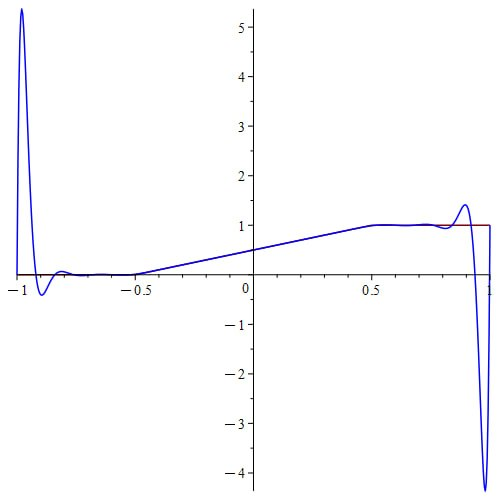
\includegraphics[width=0.7\textwidth]{figures/uni}
	\caption{Поліноміальна інтерполяція тестової функції на рівномірній сітці вузлів}
	\label{fig:uniform_interpolation}
\end{figure}

Як видно з отриманого графіка, у центральній частині інтервалу поліном відносно точно повторює форму цільової функції. Однак при наближенні до країв відрізка спостерігається яскраво виражений феномен Рунге. Інтерполянт починає здійснювати гігантські неконтрольовані осциляції, амплітуда яких значно перевищує справжні значення функції. У контексті обробки зображень такі відхилення математичної моделі є катастрофічними, оскільки вони призведуть до появи екстремальних візуальних артефактів (пересвітів або чорних провалів) на межах об'єктів.

Другим кроком є застосування альтернативної топології дискретизації — сітки Чебишева. Замість рівномірного кроку, ці вузли проєктуються з рівновіддалених точок на одиничному півколі, що забезпечує їх математично обґрунтоване згущення ближче до країв інтервалу. Результат інтерполяції тієї ж самої тестової функції за допомогою вузлів Чебишева наведено на рис.~\ref{fig:chebyshev_interpolation}.

\begin{figure}[htbp]
	\centering
	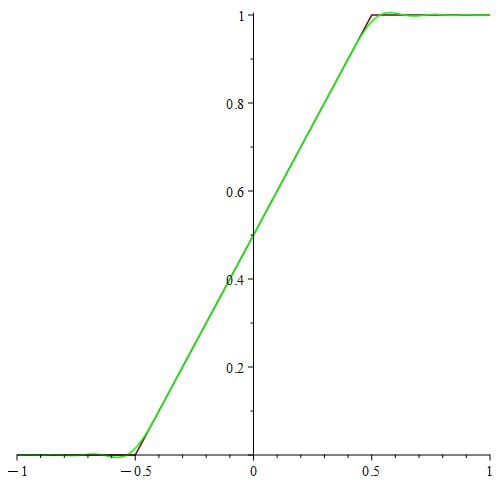
\includegraphics[width=0.7\textwidth]{figures/cheb}
	\caption{Поліноміальна інтерполяція тестової функції за вузлами Чебишева}
	\label{fig:chebyshev_interpolation}
\end{figure}

Графік наочно підтверджує ефективність чебишовського розподілу. Завдяки підвищеній щільності вузлів на краях інтервалу, поліном виявляється жорстко «зафіксованим» у найбільш проблемних зонах. Феномен Рунге повністю нівелюється, а глобальний інтерполянт ідеально та рівномірно наближає цільову функцію на всій області визначення без жодних паразитних викидів. 

Проведений порівняльний аналіз наочно демонструє зв'язок між абстрактними математичними концепціями та їх застосуванням у реальних прикладних задачах. Він беззаперечно доводить, що для побудови стабільних алгоритмів масштабування використання класичної рівномірної сітки пікселів є неприйнятним. Перехід до чебишовських вузлів гарантує структурну цілісність результату, що робить їх ідеальним базисом для подальшої розробки математичного апарату барицентричної інтерполяції.